\section{Major changes in gem5-20}
\label{sec:changes}

This section contains descriptions of some of the major changes to gem5.
There are too many changes to list.
There were XXXX commits since gem5 was released.
It is likely that major changes are missing.

\subsection[Learning gem5]{Learning gem5\footnote{By Jason Lowe-Power}}

The gem5 simulator has a steep learning curve.
Not only do new users have to navigate the 100s of different models, but they also have to understand the core of the simulation framework.
Most of the time, using gem5 in research means \emph{modifying} the simulator to change or add new models.
We found that this steep learning curve was one of the biggest impediments to productively using gem5.
There was anecdotal evidence that it would take new users \emph{years} to learn to use gem5 effectively~\cite{Power-gem5horrors-2015}.
Additionally, the only way to learn parts of gem5 was to work with a senior graduate student or to intern at a company and pick up the knowledge ``on the job''.
Many parts of gem5 were not documented except as the source code.

\emph{Learning gem5} reduces the knowledge gap between new users and experienced gem5 developers.
Learning gem5 takes a bottom up approach to teaching new users the internals of gem5.
There are currently three parts of Learning gem5, ``Getting Started'', ``Modifying and Extending'', and ``Modeling Cache Coherence with Ruby''.
Each part walks the reader through a step-by-step coding example starting from the simplest possible design up to a more realistic example.
By explaining the thought process behind each step, the reader gets a similar experience to working alongside an experienced gem5 developer.
Learning gem5 includes documentation on the gem5 website\footnote{\url{http://www.gem5.org/documentation/learning_gem5/introduction/}} and source code in the gem5 repository for these simple ground-up models.

Looking forward, we will be significantly expanding the areas of the simulator covered by Learning gem5 and creating a gem5 ``summer school''.
This ``summer school'' will mainly be an online class (e.g., Coursera), but we hope to have in-person versions of the class as well.
These classes will also be the basis of gem5 Tutorials held with major computer architecture and other related conferences.

\subsection[Testing in gem5]{Testing in gem5\footnote{by Sean Wilson and Robert R. Bruce}}

Heard back, waiting for the text.

\subsection[Updating Guest<->Simulator APIs]{Updating Guest<->Simulator APIs\footnote{By Gabriel Black}}

Haven't heard anything back, yet.

\subsection[SystemC Integration]{SystemC Integration}

While the open and configurable architecture of gem5 is of particular interest
in academia, the industry's main tool for virtual prototyping is SystemC
Transaction Level Modelling (TLM)~\cite{systemc_ieee11}. Many hardware vendors
provide SystemC TLM models of their IP and there are tools, such as Synopsys
Platform Architect\footnote{\url{https://www.synopsys.com/verification/virtual-prototyping/platform-architect.html}},
that assist in building a virtual system and analyzing it. Also, many research
projects use SystemC TLM, as they benefit from the rich ecosystem of accurate
of-the-shelf models of real hardware components. However, there is a lack of
accurate and modifiable CPU models in SystemC since the model providers want to
protect their IP. This makes the combination of gem5 with SystemC very
attractive.

\subsubsection[gem5 to SystemC Bridge]{gem5 to SystemC Bridge\footnote{By Chistian Menard, Jeronimo Castrillon, and Matthias Jung}}

SystemC TLM and gem5 were developed around the same time and are based on
similar underlying ideas. As a consequence, the hardware model used by TLM is
surprisingly close to the model of gem5. In both approaches, the system is
organized as a set of components that communicate by exchanging data packets
via a well defined protocol. The protocol abstracts over the physical
connection wires that would be used in a register transfer level (RTL)
simulation and thereby significantly increases simulation speed. In gem5,
components use \emph{master} and \emph{slave} ports to communicate to other
components, whereas in SystemC TLM, connections are established via
\emph{initiator} and \emph{target} sockets. Also, the three protocols
\emph{atomic}, \emph{timing} and \emph{functional} provided by gem5 find their
equivalent in the \emph{blocking}, \emph{non-blocking} and \emph{debug}
protocols of TLM. The major difference in both protocols is the treatment of
backpressure, which is implemented by a retry phase in gem5 and with the
exclusion rule of TLM.

\begin{figure}
    \centering
    \subcaptionbox{gem5 to SystemC\label{fig:example:gem5_to_sc}}{
      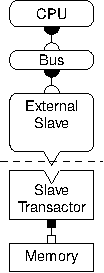
\includegraphics[height=4cm]{fig/gem5_to_systemc.pdf}
    }
    \subcaptionbox{SystemC to gem5\label{fig:example:sc_to_gem5}}{
      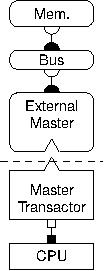
\includegraphics[height=4cm]{fig/systemc_to_gem5.pdf}
    }
    \subcaptionbox{both directions\label{fig:example:twoway}}{
      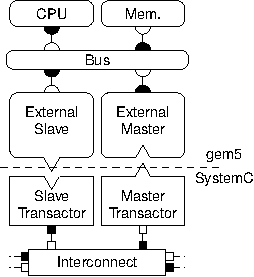
\includegraphics[height=4cm]{fig/twoway.pdf}
    }
    \caption{Possible scenarios for binding gem5 and SystemC.}
    \label{fig:gem5_tlm_example}
\end{figure}

The similarity of the two approaches enabled us to create a light-weight
compatibility layer. In our approach, co-simulation is achieved by hosting the
gem5 simulation on top of a SystemC simulation. For this, we replaced the gem5
discrete event kernel with a SystemC process that is managed by the SystemC
kernel. A set of transactors further enables communication between the two
simulation domains by translating between the two protocols as is shown in
Figure~\ref{fig:gem5_tlm_example}. This work was published
in~\cite{menard2017-system-systemc} where we documented our approach and showed
that the transaction between gem5 and TLM only introduces a low overhead of
about \(8\%\). The source code as well as basic usage examples can be found in
\texttt{util/tlm} of the gem5 repository.

\subsubsection[SystemC in gem5]{SystemC in gem5\footnote{By Gabriel Black}}

Haven't heard anything back, yet.

\subsection[ARM Fastmodel]{ARM Fastmodel\footnote{By Gabriel Black}}

Haven't heard anything back, yet.

\subsection[Cache Replacement Policies and New Compression Support]{Cache Replacement Policies and New Compression Support\footnote{By Daniel Carvalho}}

In general, hardware components frequently contain tables, whose contents are managed by replacement policies.
In gem5, multiple replacement policies are available, which can paired with any table-like structure, allowing users to carry research on the effects of different replacement algorithms in various hardware units.
Currently, gem5 supports 13 different replacement policies including several standard policies such as LRU, FIFO, and Pseudo-LRU, and various RRIPs~\cite{Jaleel2010rrip}.
This list is easily expandable to cover schemes with greater complexity as well.

The simulator also supports cache compression by providing several state-of-the-art compression algorithms~\cite{sardashti2015primer} and a default compression-oriented cache organization.
This basic organization scheme is derived from accepted approaches in the literature: adjacent blocks share a tag entry, yet they can only be co-allocated in a data entry if each of them compresses to at least a specific percentage of the cache line size.
Currently, only BDI~\cite{pekhimenko2012base}, C-Pack~\cite{chen2010c}, and FPCD~\cite{alameldeen2018opportunistic} are implemented, but the modularity of the compressors allows for simple implementation of other dictionary-based and pattern-based compression algorithms (e.g., only a few hours of development effort for a developer familiar with the code).

These replacement policies are a great example of gem5's modularity and how code developed for one purpose can be reused in many other parts of the simulator.
Current and future development is planned to increase the use of these flexible replacement policies.
For instance, we are planning to extend the TLB and other cache structures beyond the data caches to take advantage of the same replacement policies.
Additionally, although the aforementioned cache compression policies have only been applied to the classic caches, we are planning to use the same modular code to enable cache compression for the Ruby caches as well.

\subsection[Ruby Cache Model Improvements]{Ruby Cache Model Improvements}

\subsubsection[General Improvements]{General Improvements\footnote{by Nilay Vaish}}

Haven't heard anything yet.

\subsubsection[GPU Coherence Protocols]{GPU Coherence Protocols\footnote{by Blake Hectman}}

Haven't heard anything, yet.

\subsubsection[ARM Support and Extensions]{ARM Support in Ruby Coherence Protocols\footnote{by Tiago M{\"u}ck}}

Haven't heard anything, yet.

\subsection[Garnet Network Model]{Garnet Network Model\footnote{By Srikant Bharadwaj and Tushar Krishna}}

Heard back, they should be working on it.

\subsection[RISC-V ISA Support]{RISC-V ISA Support}

RISC-V is a new ISA which has quickly gained popularity since its creation in 2010, only one year before the initial gem5 release~\cite{Waterman2011riscv}.
In that time, the number of users RISC-V has grown significantly, especially in the computer architecture research community.
Thus, the addition of RISC-V as a supported ISA for gem5 is one of the main new features in the past nine years.

\subsubsection[General RISC-V ISA Implementation]{General RISC-V ISA Implementation\footnote{By Alec Rokle}}

\textbf{TODO: CITE (\url{https://carrv.github.io/2017/papers/roelke-risc5-carrv2017.pdf}) and (\url{https://carrv.github.io/2018/papers/CARRV_2018_paper_3.pdf}).}

The motivation for implementing the RISC-V ISA into gem5 stemmed from needing a way to explore architectural parameters for RISC-V designs.
At the time of implementation, the only means of simulating RISC-V was using spike (its simplified, single-cycle RTL simulator), QEMU, or full RTL simulation or emulation on FPGA.
Spike and QEMU aren’t detailed enough and RTL simulation is too time consuming for these methods to be feasible for architectural parameter exploration, and FPGA emulation is difficult to retrieve performance information from without modifying both the RTL design and executed software to track and present it.
The gem5 simulator provides an easy means of performing this type of analysis through its detailed hardware models that do not require software modification and allows for variable levels of detail.
By adding RISC-V to gem5, this type of analysis is enabled for the rapidly-growing ISA.

The implementation was done by following the divisions of the instruction set into its base ISA and extensions, beginning with the 32-bit integer base set, RV32I.
It was modeled off of the existing gem5 code for MIPS and Alpha, which are also RISC instruction sets that share many of the same operations as RISC-V.
Including support for 64-bit addresses and data (RV64) and for the multiply (M) extension mainly involved adding the new instructions and changing some parameters to expand register and data path widths.
The next two extensions, atomic (A) and floating point (F and D for single- and double-precision, respectively), were more complicated.
The A extension includes both load-reserved/store-conditional (LR/SC) sequence of instructions for performing complex atomic operations on memory and a set of read-modify-write instructions for performing simple ones.
The former two instructions had analogues in MIPS, but, at the time of implementation, gem5 did not have support for single instructions that both read and wrote memory atomically.
These instructions were implemented as a pair of micro-ops that acted like an LR/SC pair with one of the pair additionally performing the specified operation.
Floating-point instructions required many special cases to ensure correct error handling and reporting, and we were not able to implement one of the five possible rounding modes (round away from zero) RISC-V specifies for inexact calculations due to the fact that C++ does not support it.
Finally, support for the non-standard compressed (C) extension, which adds 16-bit versions of high-usage instructions, was added when it was discovered that this extension was included by default in many RISC-V software toolchains.
Its implementation required the creation of a state machine in the instruction decoder to keep track of whether the current instruction is compressed or not, to increment the PC by the correct amount based on the size of the instruction, and to handle cases where a full-length instruction crosses a 32-bit word boundary.

With this implementation, most RISC-V Linux programs are supported for execution in system-call-emulation mode.  Future work by others would then go on to improve the implementation of atomic instructions, including actual atomic read-modify-write accesses in a single instruction and steps toward support for full-system simulation.

\subsubsection[RISC-V Full System Support]{RISC-V Full System Support\footnote{By Nils Asmussen}}

Haven't heard anything back, yet.

\subsection{Predictor Improvements}

I haven't heard anything back, yet.

\subsection[GPU Compute Model]{GPU Compute Model\footnote{by Anthony Gutierrez}}

Heard back, waiting for text.
This may be a bit late due to having to run it past the lawyers.

\subsubsection[Autonomous Data-Race-Free GPU Tester]{Autonomous Data-Race-Free GPU Tester\footnote{by Tuan Ta}}

The Ruby coherence protocol tester is designed for CPU-like memory systems that implement relatively strong memory consistency models (e.g., TSO) and hardware-based coherence protocols (e.g., MESI).
In such systems, once a processor sends a memory request to memory, the request appears globally to the rest of the system.
Without knowing implementation details of target memory systems, the tester can rely on the issuing order of reads and writes to determine the current state of shared memory.
However, existing GPU memory systems are often based on weaker consistency models (e.g., sequential consistency for data-race-free) and implement software-directed cache coherence protocols (e.g., VIPER requiring explicit cache flushes and invalidations from software to maintain cache coherence).
The order in which reads and writes appear globally can be different from the order they are issued from GPU cores.
Therefore, the previous CPU-centric Ruby tester is not applicable to testing GPU memory systems.

The gem5 simulator currently supports an autonomous random data-race-free testing framework to validate GPU memory systems.
The tester works by randomly generating and injecting sequences of data-race-free reads and writes that are well synchronized by proper atomic operations and memory fences to a target memory system.
By maintaining the data-race freedom of all generated sequences, the tester is able to validate responses from the system under test.
The tester is also able to periodically check for forward progress of the system and report possible deadlock and livelock issues.
Once encountering a failure, the tester generates an event log that captures only related memory transactions related to the failure, which significantly eases the debugging process.
Tuan Ta et al. showed how the tester effectively detected bugs in the implementation of VIPER protocol in gem5~\cite{Ta2019gputesting}.

\subsection[Syscall Emulation Improvements]{Syscall Emulation Improvements\footnote{by Brandon Potter}}

Heard back, waiting for text.
This may be a bit late due to having to run it past the lawyers.

\subsection[ARM Improvements]{ARM Improvements\footnote{by Lots of People}}

Heard back, waiting for text.

Note: May want to add something about \url{https://community.arm.com/developer/ip-products/system/b/soc-design-blog/posts/simplifying-workload-modelling-with-amba-atp-engine}

\subsubsection[ARMv8 Support]{ARMv8 Support\footnote{by Giacomo Gabrielli}}

Heard back, waiting for text.

\subsection[Vector Instruction Extensions]{Vector Instructions Extensions\footnote{by Javier Setoain}}

\subsection{Internal gem5 Improvements and Features}

\subsubsection[HDF5 Support]{HDF5 Support\footnote{by Andreas Sandberg}}

Haven't heard back, yet.

\subsubsection[Python 3]{Python 3\footnote{by Andreas Sandberg and Giacomo Travaglini}}

Haven't heard back, yet.

\subsection[Flexible DRAM Controller]{Flexible DRAM Controller\footnote{by Wendy Elsasser, Matthais Jung, and others}}

Heard back, waiting for text.

\subsubsection[DRAMPower and DRAM Power-Down Modes]{\footnote{by Matthias Jung, Subash Kannoth, Omar Naji, Eder F. Zulian, Christian Weis, ...}}

Across applications, DRAM is a significant contributor to the overall system power.
For example, the DRAM access energy per bit is up to three orders of magnitude higher compared to an on-chip memory access.
Therefore, an accurate and fast power estimation is crucial for an efficient design space exploration.
DRAMPower (cite: DRAMPower: Open-source DRAM Power \& Energy Estimation Tool Karthik Chandrasekar, Christian Weis, Yonghui Li, Sven Goossens, Matthias Jung, Omar Naji, Benny Akesson, Norbert Wehn, and Kees Goossens URL: \url{http://www.drampower.info}) is an open source tool for fast and accurate power and energy estimation for several DRAM memories based on JEDEC standards.
It supports unique features like power-down, bank-wise power estimation, per bank refresh, partial array self-refresh, and many more.

In contrast to Micron’s DRAM Power estimation spread sheet (cite Micron. DDR3 SDRAM System Power Calculator), which estimates the power from device manufacturer’s data sheet and workload specifications (e.g. Rowbuffer-Hit-Rate or Read-Write-Ratio), DRAMPower uses the actual timings from the memory transactions, which leads to a much higher accuracy in power estimation.
Furthermore, the DRAMPower tool performs DRAM command trace analysis based on memory state transitions and hence, avoids cycle-by-cycle evaluation, thus speeding up simulations.

For the efficient integration of DRAMPower into gem5, we changed the tool from a standalone simulator to a library that could be used in discrete event-based simulators for calculating the power consumption online during the simulation.
Furthermore, we integrate the power-down modes into the DRAM controller model of gem5 (cite: 3.	Integrating DRAM Power-Down Modes in gem5 and Quantifying their Impact R. Jagtap, M. Jung, W. Elsasser, C. Weis, A. Hansson, N. Wehn. ACM International Symposium on Memory Systems (MEMSYS 2017), October, 2017, Washington, DC, USA) in order to provide the research community a tool for power-down analysis for a breadth of use cases. We further evaluated the model with real HPC workloads, illustrating the value of integrating low power functionality into a full system simulator.

\subsubsection[Quality of Service Extensions]{Quality of Service Extensions\footnote{by Matteo Andreozzi}}

Heard back, waiting for text.
It may be a bit late.

\subsection[Virtualized Fast Forwarding]{Virtualized Fast Forwarding\footnote{by Andreas Sandberg}}

I haven't heard anything back, yet.
Note: Cite paper ``Full Speed Ahead: Detailed Architectural Simulation at Near-Native Speed''

\subsection[gem5 and SST Integration]{gem5 and SST Integration\footnote{by Cutis Dunham}}

Haven't head back, yet.

\subsection[Memory Traces and Traffic Generator]{Memory Traces and Traffic Generator\footnote{by Andreas Hanson}}

Haven't heard back, yet.

\subsection[Classic Caches Improvements]{Classic Caches Improvements\footnote{by Nikos Nikoleris and Andreas Hanson}}

Haven't heard back, yet.

\subsubsection[Snooping Support and Snoop Filtering]{Snooping Support and Snoop Filtering\footnote{by Stephan Diestelhorst}}

Heard back, waiting for text.

\subsection[dist-gem5: Support for Distributed Computing]{dist-gem5: Support for Distributed Computing\footnote{by Gabor Dozsa}}

Haven't heard back, yet.

Note: I should probably reach out to Mohammad Alian.

Cite ``dist-gem5: Distributed Simulation of Computer Clusters'' and ``pd-gem5: Simulation Infrastructure for Parallel/Distributed Computer Systems''

\subsection[The Minor In-Order CPU Model]{The Minor In-Order CPU Model\footnote{by Andrew Bardsley}}

Haven't heard back, yet.

\subsection[Power Modeling and DVFS Support]{Power Modeling and DVFS Support\footnote{by Akash Bagdia, Stephan Diestelhorst, David Guillen-Fandos, and Anouk Van Laer}}

Haven't heard back, yet.

\subsection[Elastic Traces]{Elastic Traces\footnote{by Radhika Jagtap}}

Detailed execution-driven CPU models, like gem5, offer high accuracy, but at the cost of simulation speed.
Therefore, trace-driven simulations are widely adopted to alleviate this problem, especially for studies focusing on memory-system exploration.
However, traces with fixed time stamps always include the implicit behavior of the simulated memory system with which they were recorded.
If the memory system is changed during exploration this will lead to wrong simulation results, since an out-of-order core would react differently on the new memory system.

Ideally, trace-driven core models will mimic out-of-order processors executing full-system workloads to enable computer architects to evaluate modern systems.
Therefore, we proposed the concept of elastic traces in which we accurately capture data and load/store order dependencies by instrumenting a detailed out-of-order processor model (cite: 4.	Exploring System Performance using Elastic Traces: Fast, Accurate and Portable R. Jagtap, S. Diestelhorst, A. Hansson, M. Jung and N. Wehn. IEEE International Conference on Embedded Computer Systems Architectures Modeling and Simulation (SAMOS), July, 2016, Samos Island, Greece).
In contrast to existing work, we do not rely on offline analysis of timestamps, and instead use accurate dependency information tracked inside the processor pipeline.
We thereby account for the effects of speculation and branch misprediction resulting in a more accurate trace playback compared to fixed time traces.
We integrated a trace player in gem5 that honors the dependencies and thus adapts its execution time to memory-system changes, as would the actual CPU. Compared to the detailed CPU model, our trace player achieves a speed-up of 6-8 times while maintaining a high simulation accuracy (83-93\%), achieving fast and accurate system performance exploration.


